Pour une gestion optimale du projet, nous avons utilisé un diagramme de Gantt, permettant de répartir les tâches de manière structurée et de visualiser leur durée ainsi que leur enchaînement. 
Comme illustré dans la figure \ref{fig:gantt}, chaque tâche est associée à un intervalle de temps précis, facilitant le suivi de l'avancement et la gestion des priorités. Cet outil aide à identifier les étapes clés et à ajuster les délais si nécessaire, garantissant ainsi une coordination efficace et un déroulement fluide du notre projet.
\begin{figure}[H]
    \centering
    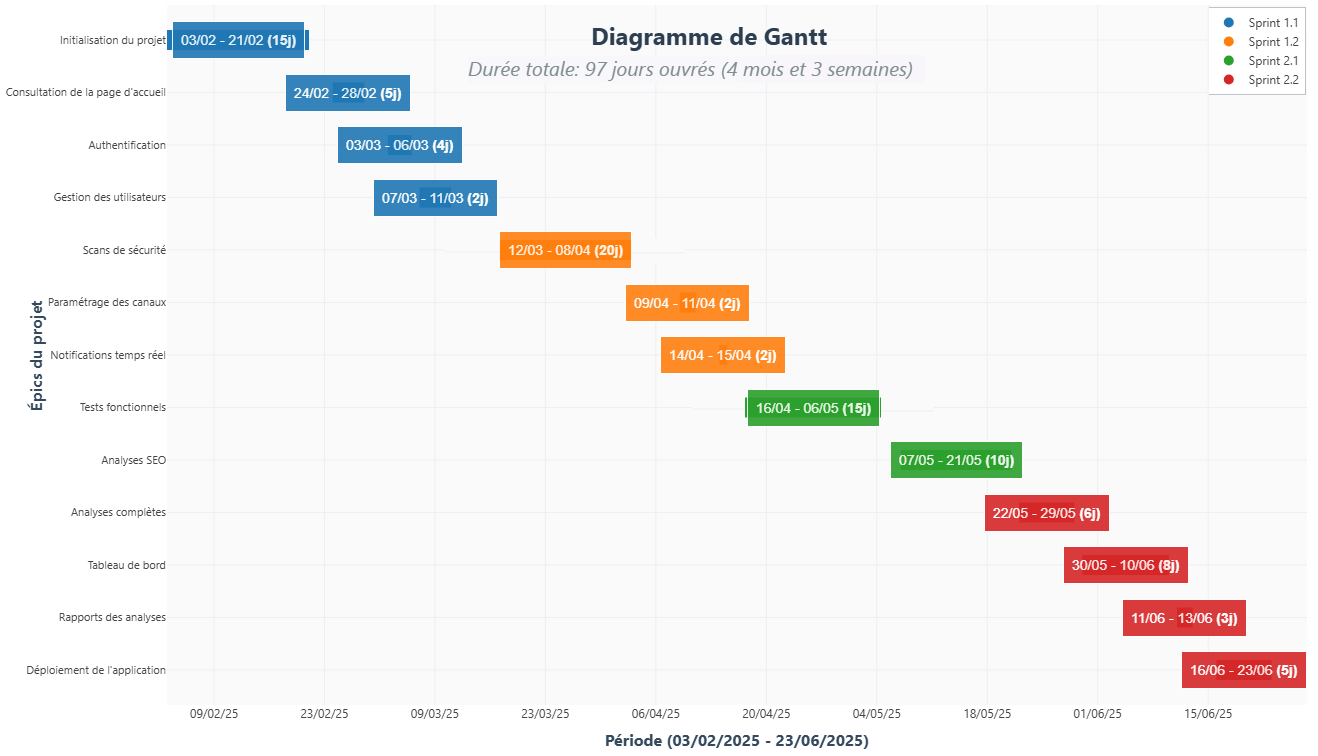
\includegraphics[width=\linewidth]{chapitres/ch2/img/gantt-last.png}
    \caption{Diagramme de Gantt}
    \label{fig:gantt}
\end{figure}
\vspace{-0.5cm}